\documentclass[12pt]{article}

\usepackage[utf8]{inputenc}
\usepackage[italian]{babel}
\usepackage{enumitem}
\usepackage{graphicx}
\usepackage{listings}
\usepackage{xcolor}
\usepackage{float}

\usepackage[backend=bibtex,sorting=none]{biblatex}
\addbibresource{references.bib}

\definecolor{codegreen}{rgb}{0,0.6,0}
\definecolor{codegray}{rgb}{0.5,0.5,0.5}
\definecolor{codepurple}{rgb}{0.58,0,0.82}
\definecolor{backcolour}{rgb}{0.95,0.95,0.92}
\lstdefinestyle{mystyle}{
    backgroundcolor=\color{backcolour},   
    commentstyle=\color{codegreen},
    keywordstyle=\color{magenta},
    numberstyle=\tiny\color{codegray},
    stringstyle=\color{codepurple},
    basicstyle=\ttfamily\footnotesize,
    breakatwhitespace=false,         
    breaklines=true,                 
    captionpos=b,                    
    keepspaces=true,                 
    numbers=left,                    
    numbersep=5pt,                  
    showspaces=false,                
    showstringspaces=false,
    showtabs=false,                  
    tabsize=2
}

\lstset{style=mystyle}

\title{Analisi di Yelp Open Dataset}
\author{
        Lorenzo Vainigli\\
        \textit{\small Corso di Intelligenza Artificiale a.a. 2019/20}\\
        \textit{\small Laurea Magistrale in Informatica}\\
        \textit{\small Università di Bologna}
}
\date{}

\begin{document}
\maketitle
\tableofcontents

\section{Introduzione}
In questo documento sono riportati i risultati dell'analisi di \textit{Yelp Open Dataset} \cite{yelp}, una base di dati che contiene informazioni su esercizi commerciali di varie categorie e presenti in diverse città degli Stati Uniti e del Canada.\newline
Il dataset è stato esaminato al fine di costruire un modello predittivo basato su una rete neurale, per produrre statistiche aggregate e trovare i valori migliori e peggiori per alcuni tipi di dato. \newline
I file di questo progetto sono disponibili nel repository dell'autore su GitHub \cite{repo}. 

\section{Dati}
I dati di \textit{Yelp Open Dataset} sono utilizzabili per uso personale, educativo o accademico, sono disponibili in formato \textit{JSON} e sono divisi in alcuni file:
\begin{itemize}
\item \textit{business.json} (153 MB): contiene le informazioni relative agli esercizi commerciali tra cui ubicazione e categoria.
\item \textit{review.json} (6,33 GB): contiene i testi delle recensioni includendo l'identificativo dell'utente che ha scritto la recensione e l'esercizio commerciale oggetto della recensione.
\item \textit{user.json} (3,27 GB): contiene i dati associati ai singoli utenti, inclusi gli identificativi degli amici.
\end{itemize}
Il database contiene anche i file \textit{tip.json}, \textit{checkin.json} e \textit{photos.json}, ma non sono stati presi in considerazione per lo sviluppo di questo progetto.
\paragraph{Caricamento dei dati}
Per motivi di performance non è stato possibile analizzare tutto il contenuto dei file \textit{review.json} e \textit{user.json}, poiché troppo grandi, mentre è stato possibile esaminare \textit{business.json} interamente.

\section{Obiettivi}
Lo scopo del progetto prevede l'analisi dei dati per studiare la loro struttura e il loro contenuto, al fine di estrapolare osservazioni interessanti su di essi. Non si tratta solo di aggregare record o trovare valori minimi, massimi o medi, ma di applicare anche tecniche di elaborazione del linguggio naturale e machine learning. In partcolare, le finalità del progetto richiedono:
\begin{enumerate}[label=T\arabic*)]
\item il riconoscimento automatico di una review positiva o negativa (sezione \ref{sec:reviews}, codice in \texttt{notebooks/reviews\_classification.ipynb});
\item il raggruppamento degli utenti in base alle loro preferenze o comportamento sulla piattaforma (sezione \ref{sec:users}, codice in \texttt{notebooks/users.ipynb});
\item il raggruppamento automatico dei locali in base a criteri di similitudine data una certa località (sezione \ref{sec:businesses}, codice in \texttt{notebooks/businesses.ipynb}).
\end{enumerate}
La cartella \texttt{notebooks} contiene altri file in cui vengono effettuate ulteriori analisi del contenuto del dataset.


\section{Strumenti}
Per conseguire gli obiettivi sopra citati i dati sono stati elaborati in \textit{Python} con ampio utilizzo delle librerie \textit{pandas}, \textit{numpy}, \textit{matplotlib} e \textit{tensorflow} sulla piattaforma \textit{Jupyter Notebook}.

\section{Classificazione delle recensioni}
\label{sec:reviews}
Grazie al dataaset \textit{review.json} è stato possibile costruire un modello predittivo basato su una rete neurale. \newline
Il file \texttt{review\_model\_test.ipynb} contiene uno script per utilizzare la rete neurale già addestrata, in cui l'utente può testare frasi a sua scelta.

\subsection{Creazione del modello}
I valori di input sono stati calcolati applicando il \textit{word embedding} al testo delle recensioni. I valori di output per ogni input sono stati calcolati in base al numero di stelle associato alla recensione e trasformato in un vettore binario per permettere al modello di effettuare una classificazione basata su categorie (es. "4 stelle" è stato codificato con il vettore [0, 0, 0, 1, 0]). \newline
Dopo numerosi tentativi, provando diverse configurazioni di livelli e parametri diversi, è stata scelta la seguente configurazione:
\lstinputlisting[language=Python]{code_snippets/nn_config.py}

\subsection{Addestramento e validazione}
Sono state selezionate le prime 10.000 recensioni, senza alcun criterio di filtraggio, effettuando una divisione 80\%-20\% per costruire, rispettivamente, training set e test set. In fase di addestramento è stato aggiunto un \textit{early stopping}. \newline
I valori di \textit{accuracy} risultanti sono 79,8\% per il training set e   63,7\% per il test set (Figura \ref{fig:run1}).
Sarebbe stato molto interessante selezionare 100.000 recensioni anziché solo un decimo di queste, ma non è stato fatto per limiti di capacità computazionali dell'elaboratore.

\begin{figure}[H]
\centering
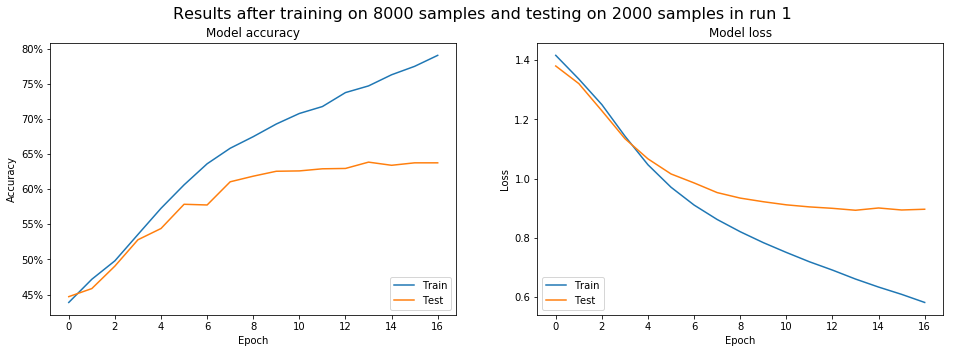
\includegraphics[width=\textwidth]{images/accuracy_loss_run1.png}
\caption{Valori di \textit{accuracy} e \textit{loss} per il primo run, ovvero prima di aver effettuato il filtraggio sui dati.}
\label{fig:run1}
\end{figure}

\subsection{Miglioramento delle performance}
Considerando che cambiando i parametri o la composizione del modello i risultati non miglioravano in modo significativo, si è scelto di effettuare un filtraggio sui dati eliminando quelli che producevano valori di \textit{loss} troppo alti. L'assunzione dietro a questa scelta sta nel fatto che questi valori di input-output potrebbero non essere molto veritieri.\newline
Per ogni istanza dei 10.000 record scelti si è calcolato il valore di \textit{loss} e si è deciso di scartare quelle che presentavano un valore più alto di 2. \newline
I valori di \textit{accuracy} risultanti dopo questa operazione sono 88,9\% per il training set e 70,3\% per il test set (Figura \ref{fig:run2}).

\begin{figure}[H]
\centering
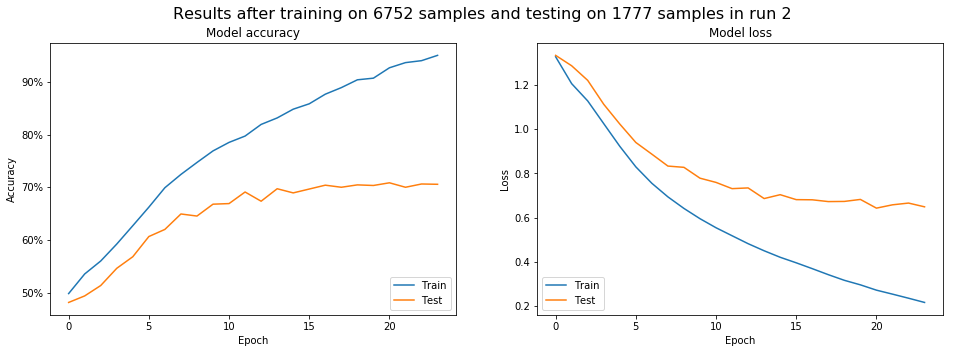
\includegraphics[width=\textwidth]{images/accuracy_loss_run2.png}
\caption{Valori di \textit{accuracy} e \textit{loss} per il secondo run, ovvero prima di aver effettuato il filtraggio sui dati dove sono stati eliminati gli esempi con valori di \textit{loss} alta.}
\label{fig:run2}
\end{figure}

\subsection{Risultati finali}
Di seguito sono riportati dei grafici che mostrano i dati sui quali si può effettuare una valutazione finale sul modello per il riconoscimento automatico di una recensione. \newline
Al fine di una classificazione tra positive e negative possiamo valutare come positive le recensioni a cui vengono attribuite 4 o 5 stelle e come negative quelle a cui ne vengono attribuite 1 o 2 stelle. Il caso delle 3 stelle è arbitrario.\newline
Osservando i grafici mostrati nelle figure \ref{fig:random_sentences_1}, \ref{fig:random_sentences_2}, \ref{fig:random_sentences_3} e \ref{fig:random_sentences_4} possiamo verificare come l'accuratezza del modello sia migliorata.
\begin{figure}[H]
\centering
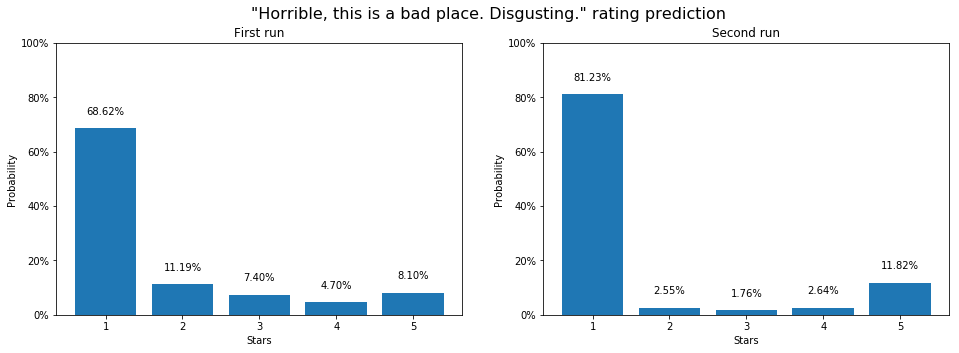
\includegraphics[width=\textwidth]{images/sent1.png}
\caption{Questa frase è sicuramente una delle peggiori che si possa scrivere a proposito di un locale. Al primo run il modello assegnava erroneamente 5 stelle ma con una notevole incertezza, mentre nel secondo run la scelta migliore (1 stella) è nettamente superiore alle altre.}
\label{fig:random_sentences_1}
\end{figure}

\begin{figure}[H]
\centering
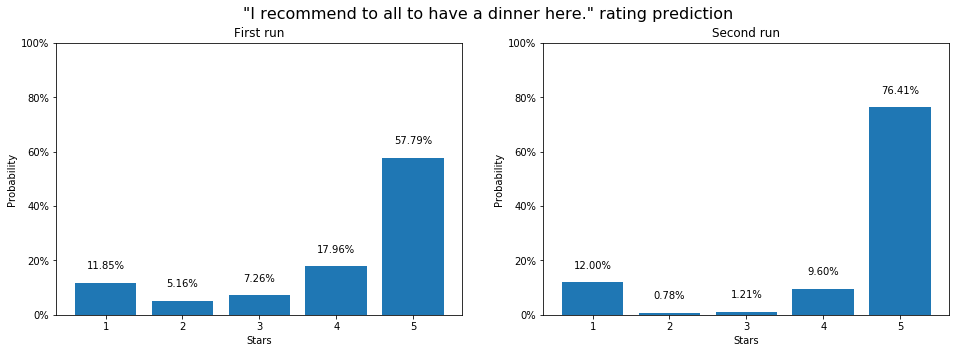
\includegraphics[width=\textwidth]{images/sent2.png}
\caption{Questa è senza dubbio una frase positiva e anche al primo run si ha una scelta netta per l'opzione 5 stelle, che comunque viene rafforzata ulteriormente nel secondo run. Sarebbe anche stato lecito aspettarsi 4 stelle.}
\label{fig:random_sentences_2}
\end{figure}

\begin{figure}[H]
\centering
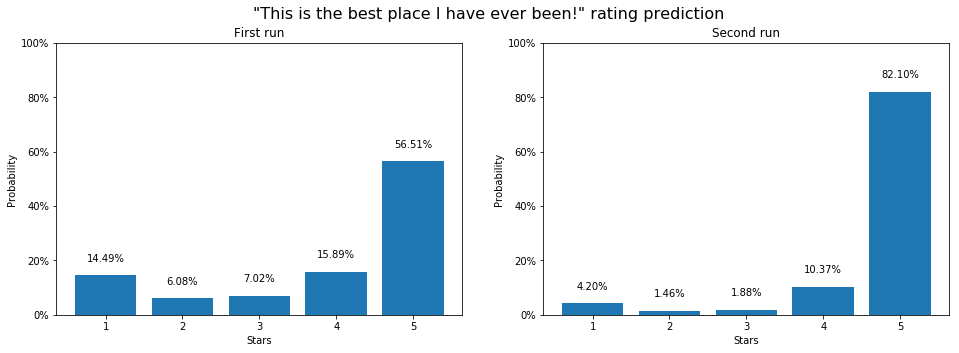
\includegraphics[width=\textwidth]{images/sent3.png}
\caption{Recensione assolutamente positiva. Già con il primo run si ha una scelta chiara, ma con il secondo l'82\% di probabilità è un risultato estremamente corretto.}
\label{fig:random_sentences_3}
\end{figure}

\begin{figure}[H]
\centering
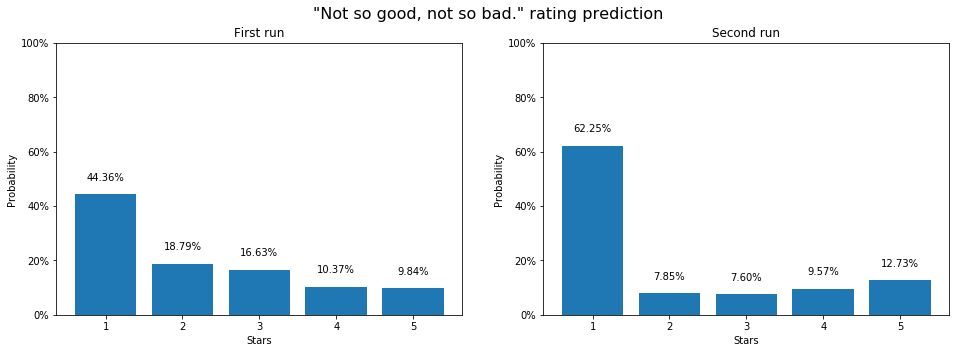
\includegraphics[width=\textwidth]{images/sent4.png}
\caption{Questa frase è una delle più interessanti poiché rappresenta un equilibrio per cui sarebbero preferibili 3 stelle (poiché si tratta della scelta media). Purtroppo in questo caso il modello non è molto accurato neanche dopo il secondo run, infatti la scelta di attribuire una stella è sicuramente sbagliata.}
\label{fig:random_sentences_4}
\end{figure}


\section{Raggruppamento degli utenti}
\label{sec:users}
Per questioni di performance e di limiti di memoria per l'elaborazione sono stati caricati sono i primi 100.000 record del file \textit{user.json}, che è composto dai campi \textit{average\_stars}, \textit{fans}, \textit{friends}, \textit{name}, \textit{review\_count}, \textit{useful}, \textit{user\_id}, e altri campi di minore importanza. \newline
Per gli utenti è stato ritenuto utile esaminare la distribuzione dei valori per i campi \textit{average\_stars}, \textit{fans} e \textit{review\_count},

\subsection{Distribuzione di \textit{average\_stars}}
Questo campo rappresenta la media delle stelle assegnate alle recensioni del singolo utente e, a differenza di tutti gli altri campi, presenta una distribuzione simile a una gaussiana.
\begin{figure}[H]
\centering
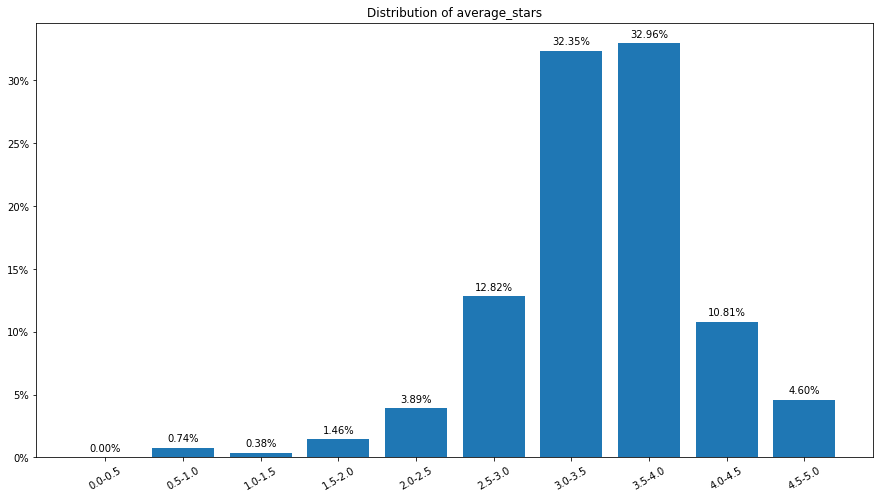
\includegraphics[width=\textwidth]{images/average_stars_distribution.png}
\caption{Distribuzione dei valori del campo \textit{average\_stars} in termini percentuali.}
\end{figure}

\subsection{Distribuzione di \textit{fans}}
Il 98,96\% degli utenti presenta un numero di fan tra 0 e 109 e l'81,71\% di questi ha meno di 6 fan. Questi valori portano alla conclusione che la user base di questo dataset è prevalentemente composta da utenti che interagiscono con una piccola cerchia di altri utenti.

\subsection{Distribuzione di \textit{review\_count}}
Questo valore dà una precisa indicazione del contributo che un utente apporta al dataset. Dall'analisi emerge che il 99,25\% degli utenti ha scritto meno di 1032 recensioni, ma è una percentuale plausibile. Molto più interessante è esaminare la segmentazione degli utenti per quanto riguarda coloro che hanno scritto meno di 100 recensioni.
\begin{figure}[H]
\centering
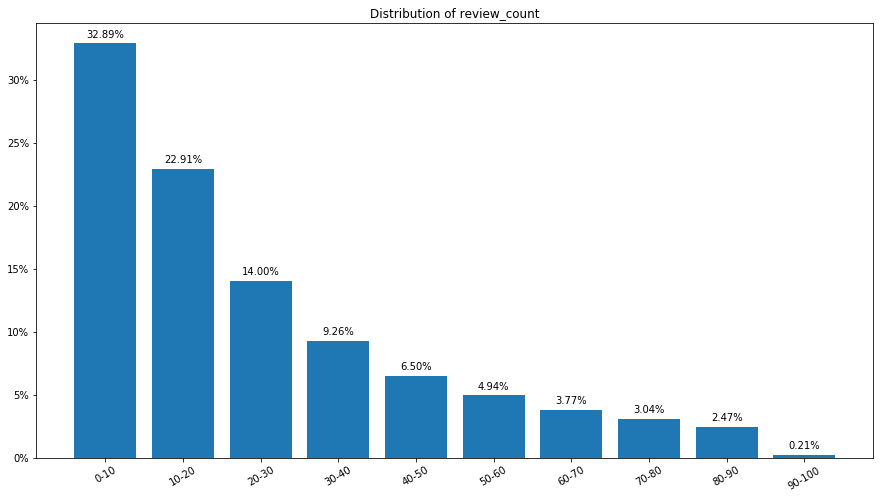
\includegraphics[width=\textwidth]{images/review_count_distribution.png}
\caption{Distribuzione dei valori del campo \textit{review\_count} per valori tra 0 e 100 in termini percentuali.}
\end{figure}

\section{Raggruppamento dei locali}
\label{sec:businesses}
Il file \textit{business.json} contiene 209.393 record, ognuno composto da 14 campi: \textit{address}, \textit{attributes}, \textit{business\_id},	\textit{categories}, \textit{city}, \textit{hours}, \textit{is\_open},	\textit{latitude} \textit{longitude}, \textit{name}, \textit{postal\_code}, \textit{review\_count}, \textit{stars} e \textit{state}.

\subsection{Migliori e peggiori}
Per questa classificazione sono stete prese in considerazione il numero di stelle assegnate a ogni esercizio commerciale e il numero di recensioni ricevuto. Si presume che, a partità di stelle, più il numero di recensioni è alto, più questo valore sia affidabile. \newline
Sono state analizzate quattro delle categorie più diffuse: \textit{Restaurants}, \textit{Shopping}, \textit{Health \& Medical} and \textit{Automotive}.\newline
\textbf{Little Miss BBQ} (Phoenix, AZ), \textbf{Brew Tea Bar} (Las Vegas, NV) e \textbf{Cocina Madrigal} (Phoenix, AZ) sono i migliori ristoranti secondo la media delle stelle e il numero di recensioni ricevute, mentre \textbf{McDonald's} (Las Vegas, NV), \textbf{KFC} (Avondale, AZ) e \textbf{McDonald's} (Fort Mill, SC) sono i peggiori.\newline
Tra i negozi catalogati come \textit{Shopping}, i migliori sono \textbf{Eco-Tint} (Las Vegas, NV), \textbf{Studio 21 Tattoo Gallery} (Las Vegas, NV) e \textbf{FINO for MEN} (Las Vegas, NV). I peggiori sono \textbf{DIRECTV} (Phoenix, AZ), \textbf{Bank of America Store and Heritage Center} (Charlotte, NC) e \textbf{Teleflora Fresh Flowers} (Las Vegas, NV). \newline
\textbf{Bangkok Thai Spa Massage} (Las Vegas, NV), \textbf{Simply Skin Las Vegas} (Las Vegas, NV) e \textbf{Richards Cosmetic Surgery, Med Spa \& Laser Center} (Las Vegas, NV) sono i luoghi migliori per la categoria \textit{Health \& Medical}. Sempre per quanto riguarda questa categoria, i luoghi peggiori sono \textbf{SilverScript Medicare} (Phoenix, AZ), \textbf{Apria Healthcare} (Henderson, NV) e \textbf{OptumCare Primary Care - Deer Valley} (Phoenix, AZ).\newline
I migliori esercizi commerciali per \textit{Automotive} sono \textbf{Eco-Tint} (Las Vegas, NV), \textbf{Precision Window Tint} (Henderson, NV) e \textbf{DC Auto Luxury Window Tinting} (Las Vegas, NV). I peggiori sono \textbf{Phoenix Car Rental} (Phoenix, AZ), \textbf{LendingTree} (Charlotte, NC) e \textbf{Seller Networks} (Las Vegas, NV).\newline
Considerando le città, \textbf{Las Vegas} è quella dove si possono trovare gli esercizi commerciali migliori, considerando queste quattro categorie, seguita da \textbf{Phoenix}.

\subsection{Categorie}
Le categorie presenti sono in totale 1.207 e le più diffuse sono \textbf{Restaurants} (13,5\%), \textbf{Shopping} (10,7\%), \textbf{Home Services} (8,2\%), \textbf{Food} (7,7\%), \textbf{Health \& Medical} (6,8\%), \textbf{Beauty \& Spas} (13,5\%), \textbf{Local Services} (5,5\%), \textbf{Automotive} (4,6\%), \textbf{Nightlife} (4,4\%) e \textbf{Event Planning \& Services} (13,5\%).

\subsection{Ubicazione}
Le città in cui si trovano i locali sono 1.306. La maggior parte dei locali si trova a \textbf{Las Vegas} (15\%), seguita da \textbf{Toronto} (10\%), \textbf{Phoenix} (10\%), \textbf{Charlotte} (5\%) e \textbf{Scottsdale} (4\%).\newline
Se si effettua il raggruppamento per Stato, allora il 29\% si trova in \textbf{Arizona (AZ)}, il 19\% in \textbf{Nevada (NV)}, il 17\% in \textbf{Ontario (ON)}, l'8\% in \textbf{Ohio (OH)} e l'8\% in \textbf{North Carolina (NC)}. I restanti sono divisi tra altri Stati.

\section{Conclusioni}
\textit{Yelp Open Dataset} è sicuramente un valido dataset se si vuole sviluppare progetti di data analysis oppure se si ha bisogno di testare la propria applicazione, ma diventa ancora più interessante in quanto può essere utilizzato, in particolare la parte che raccoglie le recensioni degli utenti, per costruire modelli di elaborazione del linguaggio naturale e di sentiment analysis.

\printbibliography[title={Riferimenti}]

\end{document}